\section{Creating the corpus}
\subsection{Downloading the files}
\label{sec:met_files}

In order to analyze the evolution of the discourse about eucalyptus, we need a large number of relevant documents. Thus, a corpus was formed through Gallica's API (the online platform of France's national library). Due to the nature of the API, we first downloaded all the metadata of the documents that mentioned the word "eucalyptus" in its text, resulting in a total of 58'157 different documents \footnote{The script was run in early March. Due to more documents being added, the number may have increased at the time of reading.}. However, due to time and API restrictions, we decided to download only a portion of the potential documents. Thus, we kept only the ones having in their metadata either a specification of its author or its publisher and mentioning the year they were published in. Figure \ref{fig:dist_filtering} shows the yearly distribution of the full corpus, compared with the filtered one. We do see that general trends prevail, while certain spikes are smoothed out. Looking more in-depth, we see that most of the filtered out documents were published in Paris, and the same for the spike in 1900. Moreover, most of the removed documents belonged to the press, meaning that, should an event happen, it would probably also be captured by another journal within the kept documents. While this means that the final corpus might not capture all local phenomena, the loss seemed reasonable, as we expected a heavier usage of the author and publisher fields. We do agree, however, that the filtering is not perfect, and looking back a random sampling would have been more relevant. Indeed, some issues arise because of the inconsistency of Gallica's metadata concerning the press, as some journals have themselves as their own publisher, whereas some do not, thus being removed from the pool of potential documents. Since this metadata decision from Gallica seems to be arbitrary and was not caught beforehand, it does present a bias in the corpus. However, given the structure of the API and time limitations that did not allow for a reevaluation of the filtering, we think the final corpus is still relevant, and the wider one (without full document information) will be used periodically if needed. 

\begin{figure}[H]
    \centering
    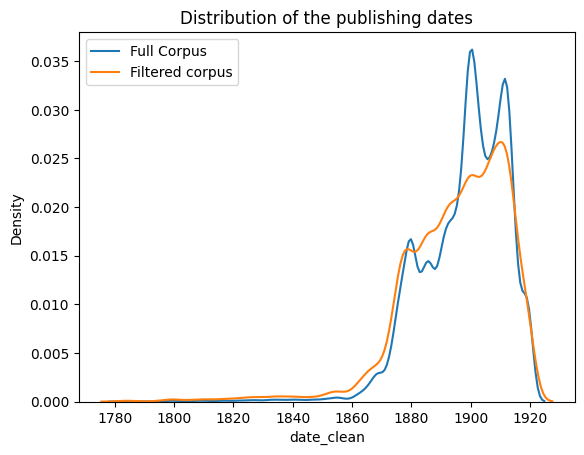
\includegraphics[width=0.5\linewidth]{Images/Figures/dist_filtering.png}
    \caption{Histogram depicting the distribution of documents in the two corpus per year.} 
    \label{fig:dist_filtering}
\end{figure}

In the end, the final corpus contains a total of 17'191 documents, ranging from 1783  to 1920. Each document possesses a title, a date of publication, either a stated author or publisher and its type (monograph or press). Moreover, the author field contains the birth and death of the authors, whereas the publisher field (even if there is no publisher stated) contains the document's place of publication. Finally, each document has its text file, directly downloaded via Gallica's API, thus relying on their own OCR model. This proves to be a slight problem, as the model used cannot be considered as "state-of-the-art" for today's standards, and a lot of errors appear, not only from misspellings but also from text structure, as their model struggles with press layout, often separating two paragraphs of the same article that should be together. 


\subsection{Enriching the metadata}

While having assembled a corpus of documents related to eucalyptus, we found that some metadata fields were either not precise enough, too precise or simply lacking. Thus, based on the existing metadata, we decided to create three new fields for our analysis: the author type (person or entity), the typology of the document (monograph, generalist press, specialized press, official press or directory) and the region where the document was published.

Concerning the author type, the general principle was to use the Spacy's entity tagging to check if the author field was a person\footnote{\cite{ines_montani_explosionspacy_2023}}. Then, should the model not detect the name of a person, the author field was matched against a list of french names. In the end, if both tests did not detect the name of a person, it was considered as an entity (for example a private journal, an association or a state). A manual test of a sample of 100 documents was conducted, showing no errors in this field.


A similar process was conducted for the type of publication. Gallica's own type field only differentiated between "monograph", "printed serial" and "directory". Keeping "monograph" and "directory" as its own entries, the challenge was differentiating between the different types of "printed serial", such as "generalist press", "official press" and "specialized press". We felt that this distinction was key for the analysis, as different types of journals have different purposes and editorial objectives. Indeed, a medicinal journal will not have the same approach as a daily newspaper, especially about the subject of eucalyptus. To differentiate between these categories, we tried to both detect keywords in the titles and use a list of known generalist newspapers. Thus, words such as "médecin, académie" were considered as "specialized", "express, eglise, gazette, dépêche" as "generalist" and "budget, procès-verbaux, officiel" as official press. A continous process of verification of the results produced by the algorithm was used to refine the results. In the end, manual verification over 100 samples only showed 1\% of error.


Finally, we regrouped the places of publication into more general regions, based on geographic and cultural factors. Thus, we have 7 "regions" in the corpus: "Île de France/Paris", "South of France", "Metropolitan France", "North Africa", "Madagascar", "Europe" and "Other". While separating Île de France and the rest of the country is reasonable given the cultural status of the capital, we need to explain the separation between "South of France" and the rest of "Metropolitan France". When discussing eucalyptus, this distinction is pertinent, as it was in the south, notably in cities such as "Montpellier" or "Toulon" \footnote{\cite[45]{doughty_eucalyptus_2000}}, that eucalyptus were planted. We decided to use the current administrative regions' borders to divide between North and South, while fully acknowledging that they are anachronistic compared to the period studied. This decision was done so that the delimitation was easier to program. In the end, the following regions were considered as "South": Nouvelle-Aquitaine, Occitanie, Auvergne-Rhône-Alpes, Provence-Alpes-Côte d'Azur and Corse. While it may not exactly align with a traditional North/South divide, it matches well enough with the regions influenced by large plantations of the tree. As with the other fields, a manual verification was conducted over 100 samples and we only found 1\% of error.



\section{Topic Modeling}
\label{sec:met_topic_modeling}

The next step in the analysis of the discourse was the implementation of a topic model, which aimed to capture the different ways eucalyptus are talked about. To do this, the BERTopic model was used, as it is currently one of the best performing open models for such an endeavor\footnote{\cite{grootendorst_bertopic_2022}}. However, we did not simply feed every document to the machine and found the corresponding topic. Indeed, the document typologies discussed in the section above have different structures, some of which would not work well for our purpose if done in such a way. For example, the generalist press might (and generally will) only have a single article about the tree within its pages. As such, capturing the topic of the whole document would not capture the information that we need. That is why it was decided to use as input every sentence where the word "eucalyptus" appeared on. There are several reasons justifying this choice. First, it allows for better capturing the different manners of discourse within a document itself. A document might conceivably talk about the origins of the plant at one point and then about its medicinal properties. A separation by sentence allows to capture both. Second, it allows to use a similar procedure for all document types, as the context window is small enough to avoid taking in irrelevant information, while seemingly wide enough to contextualize it. Finally, after performing topic modeling across different context sizes, it was found that heuristically it worked best (more sentences includes often different articles, while paragraphs are often badly detected by the OCR process, especially for press articles). However, this method might skew some distributions towards documents where the word "eucalyptus" appears very often. To mitigate this, the graphs presented throughout this paper, unless specified, have been normalized so that every document has the same weight.

The model having found 135 different topics, we decided it was best to group them into shared themes, or meta-topics. We chose to represent 10 different categories: "Geography", "Eucalyptus and Botanical Properties", "Fauna and Flora", "Malaria and Drainage", "Diseases", "Medicine and Medication", "Chemical Properties", "Industry and Manufacturing", "Institutions and Transport", "Descriptions" and "Others". An 11th "Errors" meta-topic was also created, which detected OCR errors ($\sim$7\% of all contexts). These labels were manually curated and were the fruit of a discussion between myself and this paper's supervisor. While we mainly had a bottom-up approach, regrouping topics by shared theme, we also decided to include some that we were looking for in the corpus, such as "Malaria and Drainage", as we knew that it was a key reason for eucalyptus plantations, thus not including "malaria" in the "diseases" meta-topic, and grouping it with "drainage" instead. We also decided to merge "Eucalyptus" and "Botanical Properties" as we figured that given the context, these properties were directly referencing the tree, as well as merging "Institution" and "Transport" as instead of merging the few "transport" topics into "Others", they were still relevant when linked with "Institution". However, we kept the rest of "Fauna and Flora" separated from eucalyptus, as in the context of studying the tree, it made sense to distinguish what is related to eucalyptus and what is related to the general fauna and flora. Finally, it was also decided to keep "Diseases", "Medicine and Medication" and "Chemical Properties" separated instead of a larger "Medicine" meta-topic, as they are different parts of a larger theme, that one could expect to appear in different types of documents.

Lastly, we used other sporadic methods in the following analysis. First, we have taken into account temporality, and used built-in methods in BERTopic to analyze the distribution of our topics through time. However, it takes the whole corpus into account, so when needed, a similar method was done, showing the the number of contexts associated with a topic though time. Finally, a co-occurrence graph was also constructed, with topics as nodes and the number of documents in which they appear simultaneously as weighted edges. This will also be used when needed to show the relationship between two topics.
